% !TEX root = ../main.tex
%%%%%%%%%%%%%%%%%%%%%%%%%%%%%%%%%%%%%%%%%%%%%%%%%%%%%%%%%%%%%%%%%%%%%%%
% Results I - the shape of Y(rho)
%%%%%%%%%%%%%%%%%%%%%%%%%%%%%%%%%%%%%%%%%%%%%%%%%%%%%%%%%%%%%%%%%%%%%%%

\section{Results I: the shape of \texorpdfstring{$Y(\rho)$}{Y(rho)}}
\label{sec:shape}

The Kaleckian question asks for a sign, and a sign invites a single number. The
first result of this paper is that the object being signed is a \emph{curve},
and that stating its shape first makes every later result easier to read. We
therefore begin with the response $Y(\rho)$ itself, and only then reduce it to
the frontier $\sigstar$ that the literature --- and the rest of this paper ---
uses as shorthand.

\subsection{The response is U-shaped, and the turn moves with
\texorpdfstring{$\sigma$}{sigma}}
\label{sec:turning}

$Y(\rho)$ is significantly curved. A quadratic fit places its turning point
$\rhostar$ --- the argument minimum --- \emph{inside} the swept support in 19
of 22 $(c_0,\sigma)$ cells, with $|t|$ up to $20.5$. That single fact
disqualifies any summary that compresses the response into one slope, because
on a curve that turns inside the interval the sign of a slope depends on the
interval chosen. \Cref{tab:turning} therefore reports the turn itself, together
with the quantity that proves economically decisive: which \emph{side} of it
the empirically anchored range of $\rho$ falls on.

\begin{table}[htbp]
\centering
\small
\caption{Turning point of $Y(\rho)$ and the position of the empirically
anchored range $\rho \in [0.35, 0.45]$ relative to it, at $\eta = 0$.}
\label{tab:turning}
\begin{tabular}{lrrrl}
\toprule
$\sigma$ & OLS slope & Chord & $\rhostar$ & Empirical $\rho$ lies\\
\midrule
0.30 & $+41.9$ & $+14.6$ & 0.420 & straddling\\
0.40 & $+26.8$ & $+5.2$  & 0.436 & straddling\\
0.50 & $+17.8$ & $-5.9$  & 0.462 & left of the turn\\
0.60 & $+5.6$  & $-20.7$ & 0.489 & left of the turn\\
0.70 & $-4.8$  & $-18.9$ & 0.513 & left of the turn\\
0.80 & $-11.7$ & $-33.3$ & 0.527 & left of the turn\\
1.00 & $-29.6$ & $-51.5$ & 0.569 & left of the turn\\
1.25 & $-45.3$ & $-68.8$ & 0.592 & left of the turn\\
1.50 & $-61.1$ & $-83.9$ & 0.640 & left of the turn\\
\bottomrule
\end{tabular}
\end{table}

Two regularities run down that table. The turning point \emph{rises} with the
elasticity of substitution, from $\rhostar = 0.42$ at $\sigma = 0.30$ to
$0.64$ at $\sigma = 1.50$: the more readily capital substitutes for labour, the
further retention must go before the supply channel overtakes the demand
channel it displaces. And for every $\sigma \geq 0.5$ the empirically anchored
retention rate lies to the \emph{left} of the turn --- on the falling branch.

\begin{declbox}
\emph{Retention depresses output while $\rho$ remains below a
$\sigma$-dependent threshold $\rhostar$, and expands it beyond; $\rhostar$
rises with $\sigma$, from $0.46$ at $\sigma = 0.5$ to $0.64$ at
$\sigma = 1.5$; and the empirically anchored retention rate lies below
$\rhostar$ for every $\sigma$ at or above $0.5$.}
\end{declbox}

The economic content is a statement about the \emph{margin} against the
\emph{range}. At the point where the data put $\rho$, the marginal effect of
further retention on output is negative; over a wide enough increase in $\rho$
it is positive. Both are properties of one curve, and neither is the label
``wage-led'' or ``profit-led'' applied to an economy. This formulation has the
further virtue of not depending on which interval an analyst happens to pick,
which is exactly the property a single-slope summary lacks --- and which
\cref{sec:estimator} shows to be worth $108$ design points when the two are put
side by side.

\subsection{The Cobb-Douglas case as one point on that curve}
\label{sec:baseline}

At $\sigma = 1$ the anchored range lies well to the left of the turn, and a
sweep over the canonical support reads unambiguously (\cref{tab:baseline}).

\begin{table}[htbp]
\centering
\small
\caption{Steady-state retention sweep at $\sigma = 1$, $c_0 = 1.0$.
Means over 20 seeds, 2{,}000 steps, last 50 observations.}
\label{tab:baseline}
\begin{tabular}{lrrrrrr}
\toprule
$\rho$ & $Y$ & $K$ & Employment & Unemployment & Wage share & Utilisation\\
\midrule
0.35 & 96.7 & 256.5 & 59.4 & 0.406 & 0.553 & 0.687\\
0.40 & 91.1 & 281.0 & 51.9 & 0.481 & 0.513 & 0.591\\
0.50 & 87.3 & 346.6 & 43.9 & 0.561 & 0.452 & 0.459\\
0.60 & 86.2 & 414.0 & 39.3 & 0.607 & 0.411 & 0.379\\
0.65 & 86.8 & 453.2 & 38.0 & 0.620 & 0.394 & 0.349\\
\bottomrule
\end{tabular}
\end{table}

Higher retention does exactly what the supply channel predicts to the capital
stock --- it rises from 256.5 to 453.2 --- and exactly what the demand channel
predicts to everything else. Employment falls from 59.4 to 38.0, unemployment
rises from $0.41$ to $0.62$, the wage share falls from $0.553$ to $0.394$, and
\emph{output falls}, from $96.7$ to $86.8$ (\cref{fig:retention}). This is the
strongest possible reconnection to \citeauthor{Teglio2025}'s leakage
mechanism: investment itself becomes the leak.

Note what \cref{tab:turning} adds to that reading. The output column of
\cref{tab:baseline} is not a verdict on the economy but the left branch of a U
observed at one elasticity --- and at the one value of $\sigma$ the empirical
literature explicitly rejects \citep{Knoblach2020}. Even here the turn is
inside the support, at $\rhostar = 0.569$; the sweep falls because it is
weighted toward the branch below it. Presented on its own, as an earlier draft
of this paper presented it, this table invites precisely the global label that
\cref{sec:turning} withholds.

\begin{figure}[htbp]
\centering
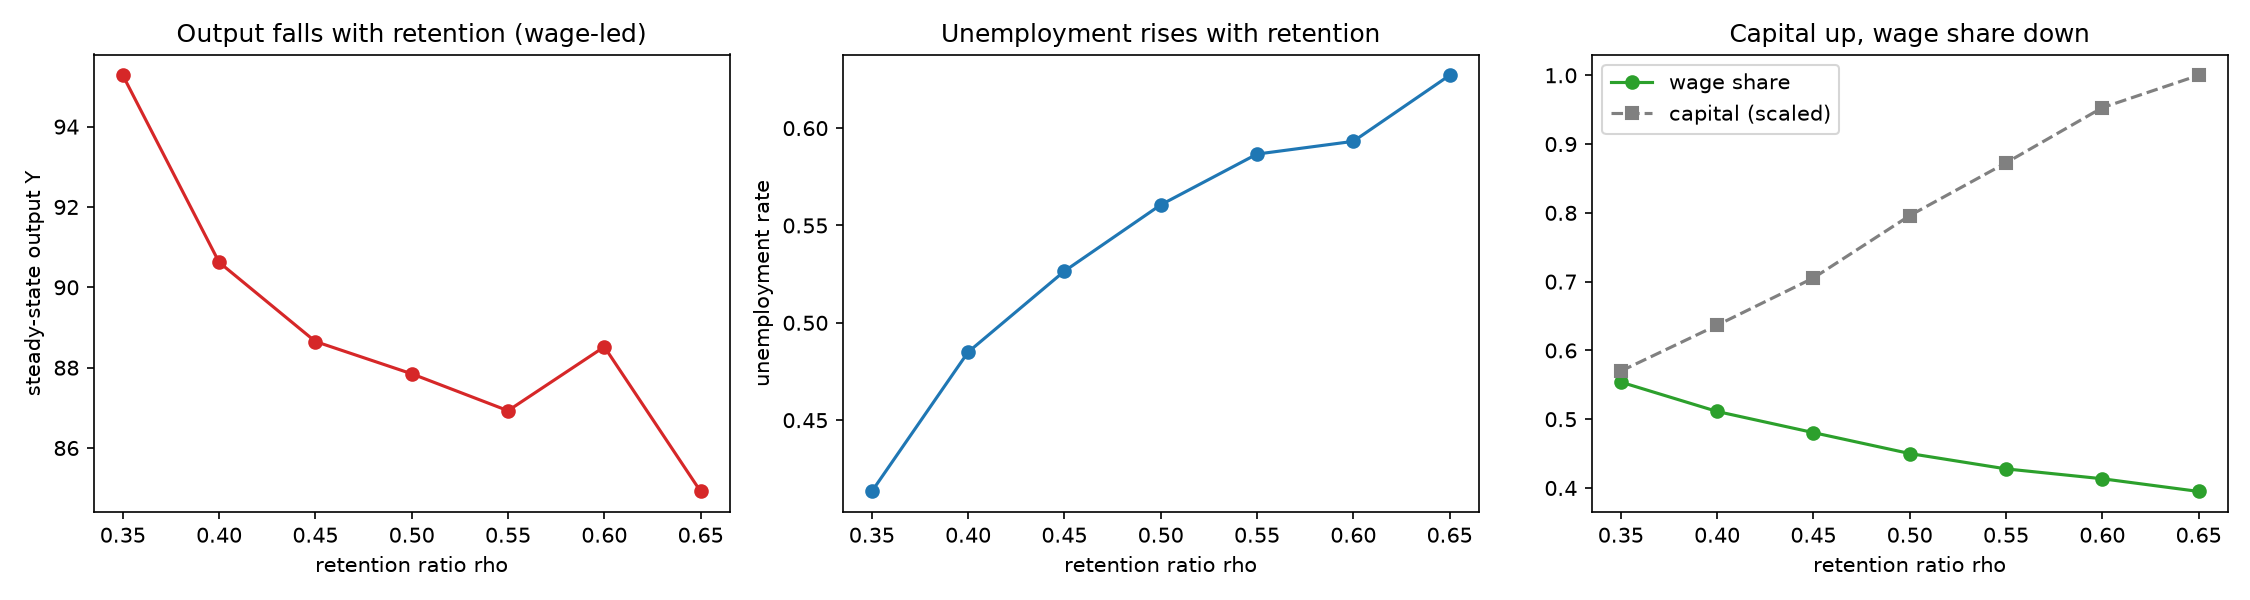
\includegraphics[width=0.82\textwidth]{retention_sweep.png}
\caption{Retention sweep at $\sigma = 1$: output falls while capital rises.
(Illustrative three-seed run; the canonical figures are those of
\cref{tab:baseline}.)}
\label{fig:retention}
\end{figure}

\subsection{\texorpdfstring{$\sigstar$}{sigma*}: the same structure read
through a single slope}
\label{sec:frontier}

Reduced to one slope per cell, the structure of \cref{tab:turning} presents as
a \emph{frontier}: the elasticity $\sigstar$ at which the estimated
$\mathrm{d}Y/\mathrm{d}\rho$ crosses zero (\cref{tab:frontier}). We retain the
reduction, because it is the form in which the comparative results of
\cref{sec:stress} and \cref{sec:government} are legible, and because it is how
the question is posed in the literature. But it is a reduction \emph{of the
curve above}, computed under the estimator declared in \cref{sec:method} --- an
OLS slope over the common viable support --- and it inherits that estimator's
choices.

\begin{table}[htbp]
\centering
\small
\caption{The sign frontier. OLS slope of the target on $\rho$ over the common
viable support; percentile bootstrap over 2{,}000 seed-resamples.}
\label{tab:frontier}
\begin{tabular}{llrlrr}
\toprule
$c_0$ & Target & $\sigstar$ & 95\% CI & Resamples with no sign change
& $P(\sigstar > 0.60)$\\
\midrule
1.0 & $Y$ & 0.654 & $[0.616,\,0.691]$ & 0\% & 99.8\%\\
1.0 & $U$ & 0.314 & $[0.300,\,0.325]$ & 0\% & 0\%\\
2.0 & $Y$ & 0.941 & $[0.918,\,0.963]$ & 0\% & 100\%\\
2.0 & $U$ & 0.450 & $[0.444,\,0.456]$ & 0\% & 0\%\\
\bottomrule
\end{tabular}
\end{table}

Two readings follow, and they pull in opposite directions.

\begin{itemize}
  \item \textbf{The empirical range sits below the frontier.} With $\sigma \in
  [0.40, 0.60]$ and $\sigstar = 0.654$, the empirically supported region has a
  positive whole-support slope: conditional on everything else being at its
  default, retention raises output across the swept range where the data put
  $\sigma$. Read against \cref{tab:turning} this is the right branch of the U
  dominating the fit --- not a contradiction of the negative margin at the
  anchored $\rho$, but the same curve summarised over a wider interval.
  \item \textbf{Unemployment has a different frontier.} $\sigstar_U \approx
  0.31$--$0.45$ lies well below $\sigstar_Y$. In the band $\sigma \approx
  0.3$--$0.7$, output \emph{and} unemployment rise together --- growth with
  technological unemployment, a configuration that neither ``wage-led'' nor
  ``profit-led'' describes. \Cref{fig:frontier} maps the sign over the whole
  $(\sigma,\rho)$ grid.
\end{itemize}

\begin{figure}[htbp]
\centering
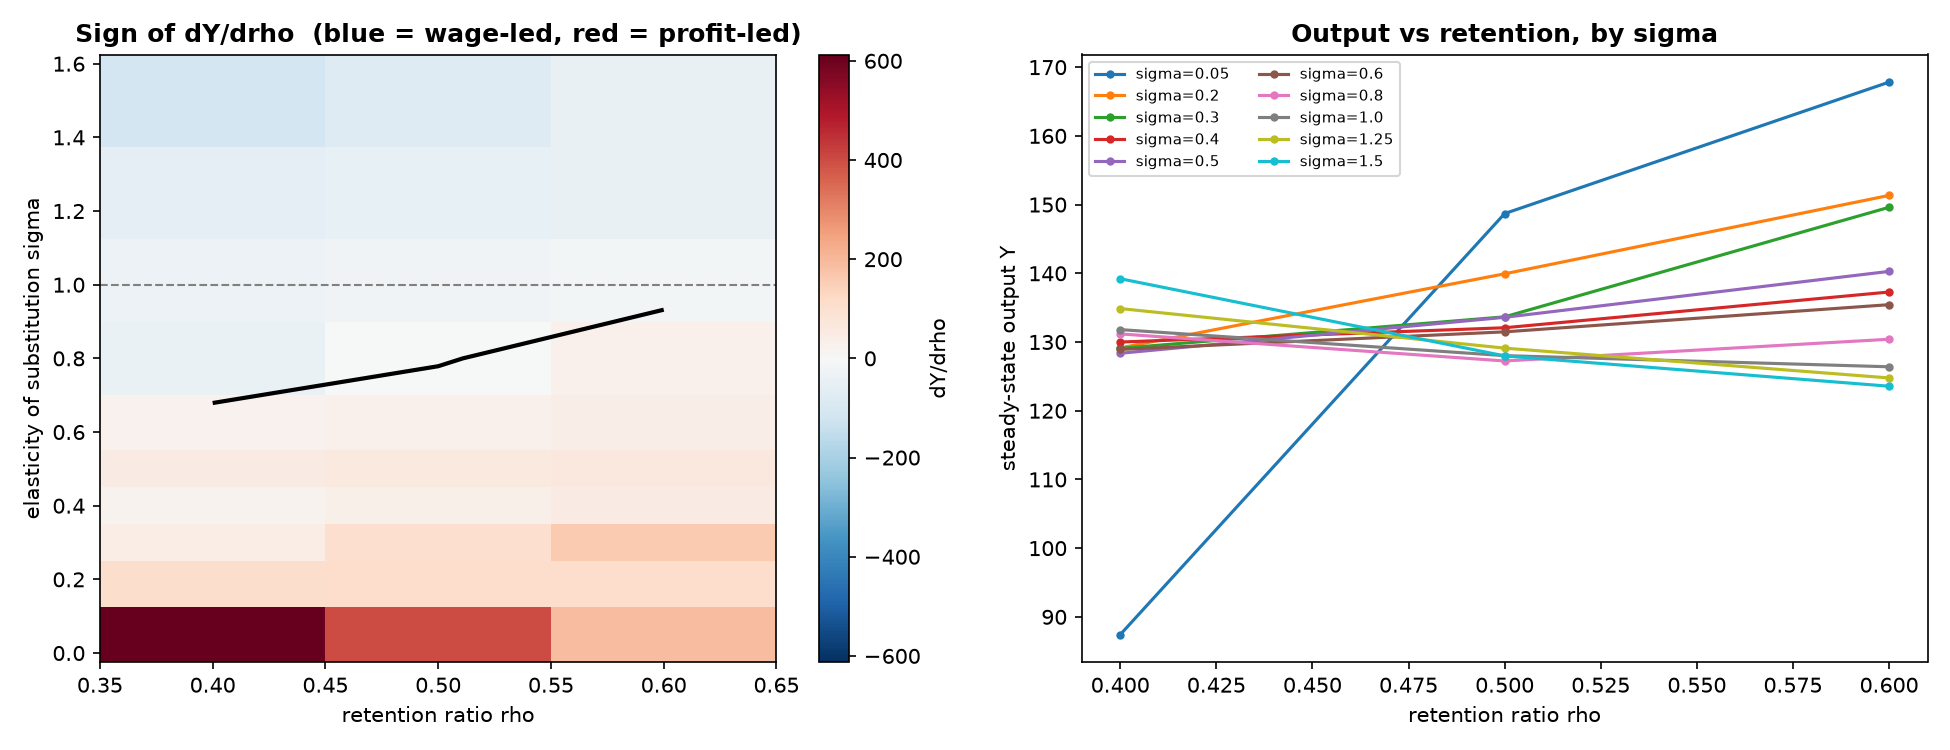
\includegraphics[width=0.82\textwidth]{ces_sign_frontier.png}
\caption{Sign of $\mathrm{d}Y/\mathrm{d}\rho$ over the $(\sigma,\rho)$ grid.}
\label{fig:frontier}
\end{figure}

\subsection{What \texorpdfstring{$\sigstar$}{sigma*} is conditional on}
\label{sec:frontier-fragility}

Reporting $\sigstar = 0.654$ as a point estimate would overstate what has been
measured. Beyond the curvature established in \cref{sec:turning}, two further
conditioning dimensions move it materially. The \textbf{choice of support}: at
$c_0 = 1.0$, $\sigstar$ ranges from $0.46$ on $\rho \in [0.35, 0.55]$ to
$0.94$ on $\rho \in [0.45, 0.65]$. And the \textbf{choice of normalisation
anchor}: moving it from $\rho = 0.40$ to $\rho = 0.50$ shifts $\sigstar$ from
$0.84$ to $0.64$ --- precisely the sensitivity \citet{Temple2012} warns of,
reported here rather than suppressed.

Both are consequences of the curvature, not independent fragilities. Where the
labels ``wage-led'' and ``profit-led'' appear in what follows they are used as
local descriptions of one side of the turn, under the estimator declared in
\cref{sec:method}; the convention is fixed here and not restated at each use.
